% Drawing 67/01-4 -- folder 67, batch 01, archive page 5 (PDF page 6).
% Transcription: feuillet de croquis, formules éparses et dessins dans tous les sens ; on n'en donne que les formules
% Kind: page of sketches (surfaces, pants, spheres). Method 2 (schematic redraw from the facsimile). Status: partial.
% Notes: Whole page; most of it written upside down. Redrawn schematically: a Y-shaped piece (pair of pants) with a bar, a small disc on a stalk, a crescent, a large circle (top); the long ink line with its step and the shorter line under it; the blob with crescents and the vertical stroke (bottom middle); a sphere with two meridian arcs (bottom right); the long faint diagonals and the faint pencil sketches in the upper left only indicated. All formulas (given in the transcription) are left out.
% Coordinates: 1 unit = 1 mm = 1/100 of the crop width (bbox in page fractions: [0.05, 0.05, 0.95, 0.88]).
% Redrawn by Claude (claude-opus-5-5), issue #73, 2026-11-07; not checked by a human; not compiled (no TeX in the session).
% Rights: reproduces part of the work -- behind RENDER_TRANSCRIPTS, never published by itself.
\documentclass[tikz,border=3pt]{standalone}
\usepackage{amsmath,amssymb}
\usetikzlibrary{patterns,arrows.meta}
\tikzset{pencil/.style={black!45}, struck/.style={black!35}, mark/.style={circle,draw,inner sep=1.3pt}, pt/.style={circle,fill,inner sep=0.9pt}, opt/.style={circle,draw,fill=white,inner sep=1.1pt}}
\begin{document}
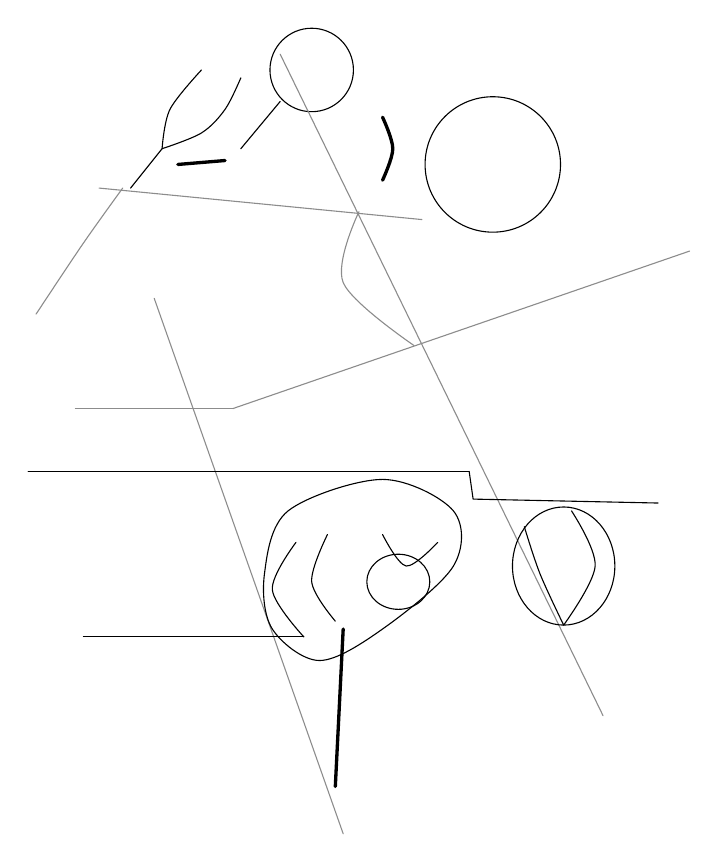
\begin{tikzpicture}[x=1mm,y=1mm,line cap=round,line join=round,font=\scriptsize]
\draw (18,-36) -- (22,-31);
\draw plot[smooth, tension=0.55] coordinates {(22,-31) (23,-26) (27,-21)};
\draw plot[smooth, tension=0.55] coordinates {(22,-31) (27,-29) (30,-26) (32,-22)};
\draw[very thick] (24,-33) -- (30,-32.5);
\draw (32,-31) -- (37,-25);
\draw (41,-21) circle[radius=5.3];
\draw[very thick] plot[smooth, tension=0.55] coordinates {(50,-27) (51.3,-31) (50,-35)};
\draw (64,-33) circle[radius=8.6];
\draw[pencil] (37,-19) -- (78,-103);
\draw[pencil] (21,-50) -- (45,-118);
\draw[pencil] (11,-64) -- (31,-64);
\draw[pencil] (31,-64) -- (89,-44);
\draw[pencil] plot[smooth, tension=0.55] coordinates {(6,-52) (12,-43) (17,-36)};
\draw[pencil] (14,-36) -- (55,-40);
\draw[pencil] plot[smooth, tension=0.55] coordinates {(47,-39) (45,-48) (54,-56)};
\draw (5,-72) -- (61,-72);
\draw (61,-72) -- (61.5,-75.5) -- (85,-76);
\draw (12,-93) -- (40,-93);
\draw plot[smooth cycle, tension=0.55] coordinates {(35,-85) (38,-77) (50,-73) (59,-77) (59,-84) (50,-92) (42,-96) (36,-92)};
\draw plot[smooth, tension=0.55] coordinates {(39,-81) (36,-87) (40,-93)};
\draw plot[smooth, tension=0.55] coordinates {(43,-80) (41,-86) (44,-91)};
\draw (52,-86) ellipse[x radius=4, y radius=3.5];
\draw plot[smooth, tension=0.55] coordinates {(50,-80) (53,-84) (57,-81)};
\draw[very thick] (45,-92) -- (44,-112);
\draw (73,-84) ellipse[x radius=6.5, y radius=7.5];
\draw plot[smooth, tension=0.55] coordinates {(68,-79) (70,-85) (73,-91.5)};
\draw plot[smooth, tension=0.55] coordinates {(74,-77) (77,-84) (73,-91.5)};
\end{tikzpicture}
\end{document}
